\documentclass{article}
\usepackage[italian]{babel}
\linespread{1.3}
\usepackage[a4paper, total={6in, 8in}]{geometry}
\usepackage{graphicx,multicol,hyperref,wrapfig}
\setlength\columnsep{30pt}
\hypersetup{
    colorlinks=true,
    linkcolor=black,
    filecolor=magenta,
    urlcolor=cyan,
    pdftitle={Relazione OsteoWeb}
}

\title{OsteoWeb}
\author{Lorenzo Albertin: lorenzo.albertin@studenti.unipd.it 2076438
        \\Federica Bolognini: federica.bolognini@studenti.unipd.it 2011881
        \\Matteo Marangon: matteo.marangon.4@studenti.unipd.it 2009094
        \\Nicholas Meneghin: nicholas.meneghin@studenti.unipd.it 2043952}
\date{A.A. 2024/2025}

\begin{document}

\begin{figure}
    \centering
    
\includegraphics[width=0.3\textwidth]{immagini/unipdlogo.png}
\end{figure}
\maketitle
\begin{figure} [h]
    \centering
    
\includegraphics[width=0.1\textwidth]{immagini/sm_logotipo.png}
\end{figure}
\begin{center}
    Link al progetto sul server tecweb:
    \href{http://tecweb.studenti.math.unipd.it/lalberti}{http://tecweb.studenti.math.unipd.it/lalberti}\newline\newline\newline % verificare link per la consegna
    Credenziali per l'accesso: \newline\newline
    \begin{tabular}{c | c | c}
    username & admin & user \\ 
    password & admin & user
    \end{tabular}
\end{center}
\newpage

\tableofcontents
\newpage

\section{Introduzione}
\subsection{Abstract}
Questa relazione illustra lo sviluppo del sito web realizzato per l'\textbf{osteopata Samuele Masiero}.
\\L'obiettivo primario è stato fornire una risorsa online completa e accessibile, in cui gli utenti possano reperire con facilità tutte le informazioni necessarie riguardo alle terapie offerte, le sedi e gli orari delle cliniche, nonché i recapiti per un contatto diretto o per prenotare in modo semplice una visita. Nella realizzazione del progetto sono stati presi in considerazione gli standard dello sviluppo web al fine di ottenere un sito che risulti fruibile per un ampio spettro di utenti, adeguandosi alle esigenze di accessibilità e usabilità.
\subsection{Analisi del target} \label{target}
Il sito si rivolge ad ogni persona che sia interessata ad una visita presso un osteopata e qualsiasi potenziale cliente che stia cercando una soluzione ad un vario genere di dolori. Si ritiene che la grande maggioranza dei visitatori del sito appartenga all'area geografica nei pressi delle sedi dell'osteopata e sia in grado di comprendere la lingua italiana. L'utenza di riferimento per questo sito sottende quindi un ampio range di età e conoscenza dei device tecnologici che abbiamo cercato di coprire in maniera quanto più semplice ma elegante possibile. Si suppone comunque una conoscenza minima della navigazione web e il raggiungimento della maggiore età in caso di prenotazione.
\newline A questo proposito, il sito è stato presentato ad alcune persone con un'alfabetizzazione informatica intermedia per testare delle componenti di web design e usabilità. La versione desktop è stata solo lievemente ritoccata, ma il feedback più sostanzioso ci è stato restituito in merito alla versione mobile, probabilmente per la maggiore familiarità in questo ambiente. Questo processo ci è stato molto utile per ricollocare alcuni elementi dell'interfaccia e riformulare alcune sezioni.
\subsection{Caratteristiche degli utenti}
Ci sono tre tipologie di utenti nel sito:
\begin{itemize}
    \item \textbf{Utenti registrati} (user o altro username). Gli utenti registrati possono navigare nella maggior parte delle pagine del sito. Possono leggere le ultime notizie, cercare i contatti e navigare tra le varie pagine. I vantaggi di eseguire la registrazione sono l'auto-completamento dei dati personali in fase di prenotazione e l'accesso alla dashboard per verificare l'accettazione (o eventualmente disdire) le proprie prenotazioni.
    \item \textbf{Utenti non registrati}. Abbiamo voluto fare in modo che il sito fosse molto simile e godibile anche per gli utenti che preferiscono non effettuare la registrazione, pertanto essi possono accedere liberamente alle stesse pagine, inclusa la prenotazione, salvo la dashboard che naturalmente richiede la registrazione (vedi [\ref{dashboard}]). In questo caso gli utenti dovranno inserire manualmente i propri dati in caso di prenotazione e riceveranno le comunicazioni strettamente legate alla loro seduta via email.
    \item \textbf{Amministratore} (admin). Oltre a quanto precedentemente descritto per gli utenti, l'admin possiede altri privilegi: visualizzare ogni pagina del sito; controllare le prenotazioni dei clienti dalla propria dashboard, accentandole o rifiutandole; inserire, modificare o eliminare le news.
\end{itemize}
\subsection{Compatibilità e requisiti di funzionamento}
Il sito web è stato testato da browser Chrome, Edge, Firefox, Safari, al fine di individuare e risolvere eventuali anomalie legate allo stile, al layout o alle funzionalità interattive. Per massimizzare la fruibilità il codice è stato scritto secondo gli standard più recenti (HTML5, CSS 3 e JavaScript), mantenendo comunque un certo grado di retrocompatibilità con un leggero supporto ad XHTML. Il design è responsive, quindi il layout si adatta automaticamente a schermi di dimensioni differenti, dai dispositivi mobili ai monitor desktop di ampie dimensioni. Inoltre, per consentire la visualizzazione dei contenuti anche nei browser che non supportano o hanno disabilitato JavaScript, è stato previsto l'utilizzo del tag \verb|<noscript>|. In questo modo è possibile continuare a fornire un livello minimo di fruizione del sito, pur senza alcune funzionalità interattive.
\section{Pagine ed elementi}
\subsection{Homepage}
La homepage ha l'intenzione di offrire una panoramica sui trattamenti proposti da Samuele Masiero per fornire un'idea immediata anche all'utente che visita il sito senza particolari conoscenze o intenzioni (analogamente al caso della pesca con la rete nella metafora della pesca) oppure all'utente che conosce l'argomento ma vuole saperne di più (nella stessa metafora, la trappola per aragoste). L'utente che invece cerca un'informazione precisa o, ad esempio, è intenzionato ad effettuare una prenotazione, troverà l'informazione che gli serve immediatamente nel menu, come spiegato nella sezione \ref{headermenu}.
\newpage
\subsection{Header e menu} \label{headermenu}
L'header resta principalmente invariato per tutte le pagine ed è composto dal logo e dalle voci del menu. Il pulsante che abbiamo voluto risaltare maggiormente è quello di prenotazione, poiché riteniamo che sia una pagina necessaria da raggiungere rapidamente da qualsiasi altro punto del sito, pertanto l'abbiamo posizionato come prima voce del menu e all'interno di un bottone. La voce "Account" porta alla pagina di accesso tramite login o registrazione, oppure alla propria dashboard qualora fosse già stato eseguito l'accesso e si trova come ultima voce per convenzione esterna. Tutte le altre voci portano alla rispettiva pagina e sono disposte nell'ordine di importanza che vogliamo comunicare all'utente. La breadcrumb è stata inserita come da requisiti WCAG per aiutare l'utente a restare sempre orientato all'interno del sito. La sua implementazione è piuttosto tradizionale e mostra il percorso tramite cui si giunge alla pagina corrente.
\subsection{Footer}
Il footer è diviso in due colonne separate dal logo dell'osteopata, contenenti i contatti e i social di Samuele Masiero, in modo tale che siano sempre facilmente reperibili dove l'utente si aspetta di trovarli come convenzione esterna.
\subsection{Account e Dashboard} \label{dashboard}
Le pagine prevedono una semplice schermata di login/registrazione che permette di accedere ad una dashboard dalla quale si possono visionare le proprie prenotazioni all'interno di una tabella accessibile. Quest'ultima è stata sviluppata con cura utilizzando \verb|aria-describedby|, \verb|<thead>|, \verb|<tbody>|, le intestazioni sono accompagnate da \verb|scope| ed è stata provata con uno screen reader. Abbiamo scelto di estendere l'utilizzo della tabella verticale anche all'utilizzo da desktop, per evitare lo scorrimento orizzontale, data la grande quantità di attributi necessari.
\subsection{Prenotazione}
Questa pagina è dedicata alla prenotazione di un appuntamento da parte di un utente registrato o meno. Trattandosi di una pagina quasi interamente dedicata ad un form, abbiamo utilizzato tag \verb|<fieldset>| per raggruppare i campi e attributi \verb|aria| per eseguire controlli client-side accessibili.
\subsection{Chi Sono}
Qui si può avere una prima conoscenza con l'osteopata, leggendo un suo breve background che può fornire contesto e familiarità ad un nuovo utente che vuole scoprire con chi sta per interfacciarsi. Abbiamo cercato di mantenere la parte biografica asciutta ma interessante e abbiamo aggiunto una timeline della vita per riassumerla ulteriormente in brevi punti.
\subsection{Sedi}
Questa pagina fornisce un'idea all'utente sulla posizione delle due sedi dell'osteopata, sulla loro posizione e i loro contatti. Abbiamo scelto una mappa di Google Maps per la maggiore accessibilità garantita. Sia le immagini delle sedi che le mappe sono dotate di attributi \verb|alt| per fornire a tutti una descrizione esaustiva dell'ambiente e della sua posizione.
\subsection{News}
Le notizie della clinica hanno lo scopo di avvisare l'utente qualora vi fossero modifiche ai giorni o agli orari di ricevimento e allo stesso tempo fornire un valore aggiunto tramite consigli e brevi inserti che si auspica vengano recepiti in maniera interessata o incuriosita.
\subsection{Pagine di conferma}
Dopo aver effettuato una prenotazione o aggiunto una notizia, si verrà indirizzati alla rispettiva pagina di conferma, che rassicura l'utente sul successo dell'operazione appena compiuta e lo invita a tornare ad una pagina piuttosto che ad un'altra, a seconda della propria esigenza successiva.
\newpage
\section{Progettazione}
\subsection{Fase prototipale} \label{faseprototipale}
Inizialmente il gruppo ha svolto in maniera collettiva la fase progettuale e prototipale del sito: ogni membro ha dato un apporto personale alla struttura principale del sito, valutando che pagine inserire e come implementarle. In seguito si è scelto di affidare mansioni più specifiche a ciascun componente, riportate nel dettaglio nella sezione [\ref{ruoli}], senza escludere però situazioni di cooperazione in cui un membro ha fornito aiuto ad un compagno qualora vi fosse necessità di confronto o supporto.
\newline Di seguito alcune bozze delle varie pagine del sito web, realizzate con Balsamiq, rispettivamente nelle loro versioni \hyperref[fig:mockup_mobile]{mobile} e \hyperref[fig:mockup_desktop]{desktop}:
\begin{figure} [h] \label{fig:mockup_mobile}
    \centering
    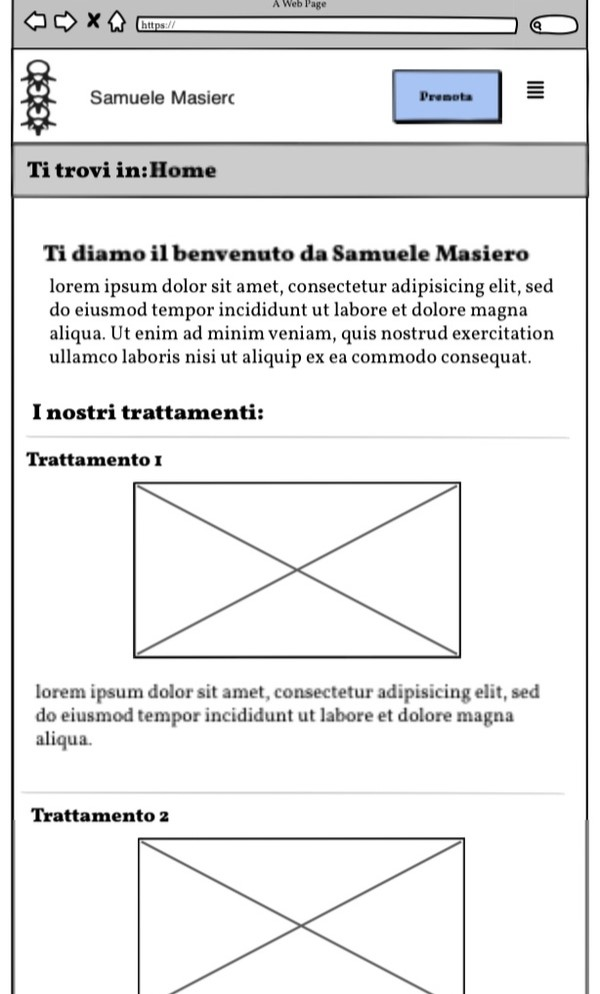
\includegraphics[width=0.3\textwidth]{immagini/homepage_mobile.jpg}
    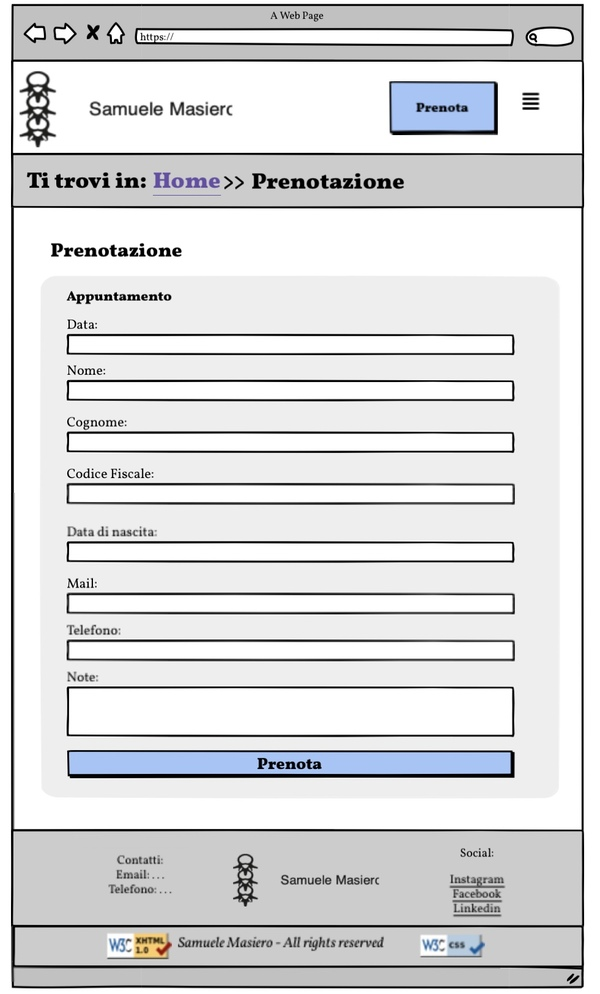
\includegraphics[width=0.3\textwidth]{immagini/prenotazione_mobile.jpg}
    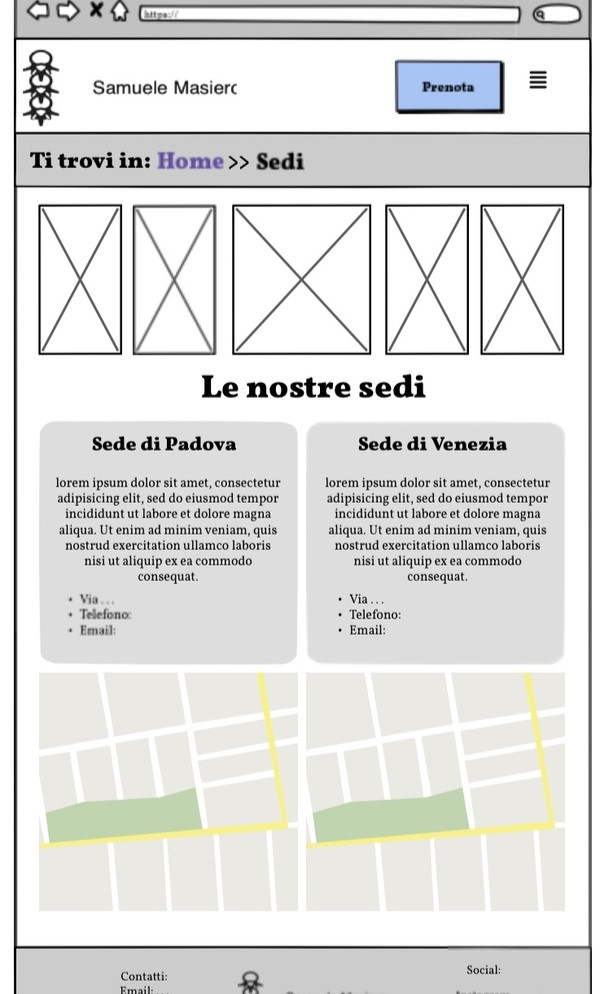
\includegraphics[width=0.3\textwidth]{immagini/sedi_mobile.jpg}
    \caption{Prototipi della versione mobile}
\end{figure}
\\Rispetto ai mockup iniziali, le pagine qui mostrate nella loro versione mobile non hanno subito modifiche sostanziali ma solo estetiche: la pagina prenotazione è stata abbellita e inquadrata in categorie di riempimento e la pagina sedi ha immagini statiche. Nonostante queste fossero inizialmente pensate come un carosello dinamico, abbiamo preferito la semplicità di una pagina statica per evitare problemi alle persone con disturbi dell'attenzione o altre problematiche cognitive.
\begin{figure} [h] \label{fig:mockup_desktop}
    \centering
    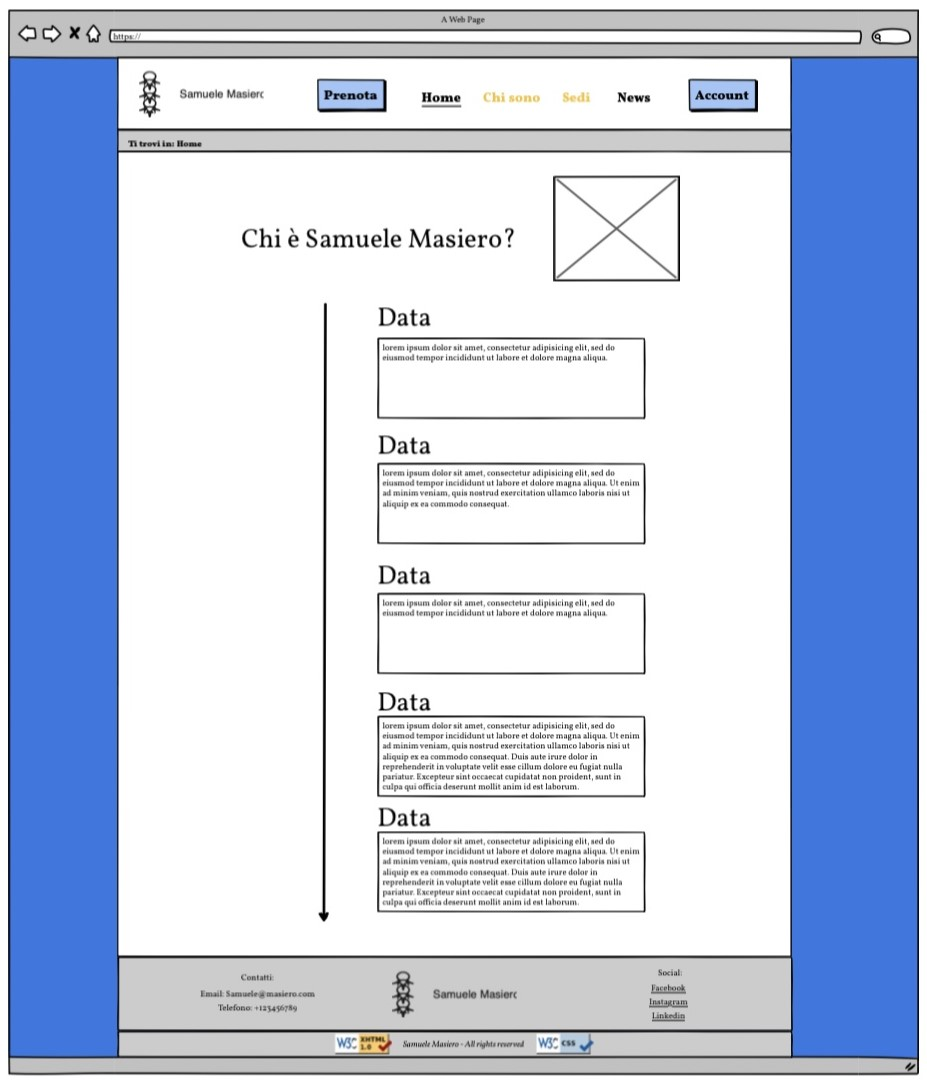
\includegraphics[width=0.35\textwidth]{immagini/about_desktop.jpg}
    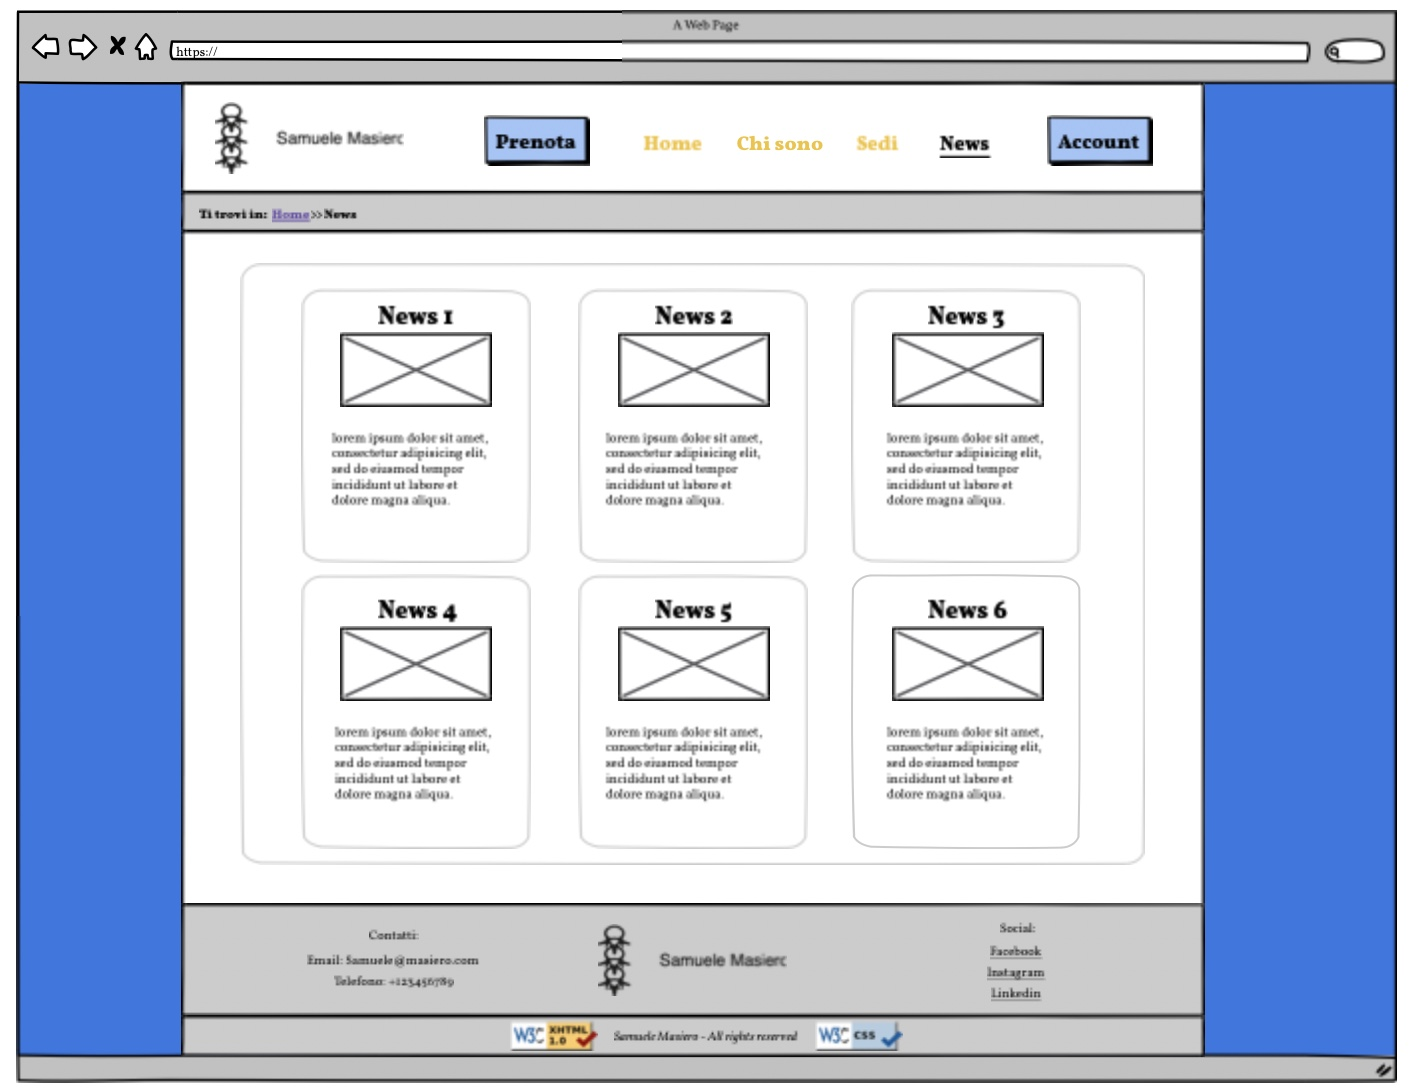
\includegraphics[width=0.54\textwidth]{immagini/news_desktop.jpg}
    \caption{Prototipi della versione desktop}
\end{figure}
\\D'altro canto, in questi mockup desktop si possono notare differenze più importanti. La pagina "Chi Sono" è stata ripensata in una biografia più riassuntiva e gli eventi della vita di Samuele sono stati concentrati in una timeline che sperabilmente sia più accattivante. Le news invece sono disposte in colonna anziché all'interno di box per migliorare il processo di lettura: nella Homepage l'utente vedrà l'anteprima di una news e qualora fosse interessato potrà raggiungere direttamente la news completa, trascritta nella sua interezza in un paragrafo dedicato.
\subsection{Struttura gerarchica} \label{gerarchia}
Durante la progettazione del sito, abbiamo mantenuto una gerarchia al suo interno che si sviluppasse quanto più orizzontalmente possibile, pur nella sua semplicità, evitando strutture annidate che rischiassero di portare l'utente ad una situazione di disorientamento e un'eccessività di click per raggiungere una determinata sezione di interesse. Come visibile nella figura \ref{fig:gerarchia}, grazie ad un numero contenuto di pagine esse sono quasi tutte raggiungibili dalla Home, ad eccezione della Dashboard che richiede l'accesso.
\begin{figure} [h] 
    \centering
    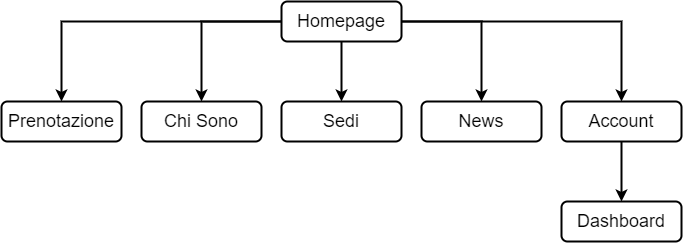
\includegraphics[width=0.7\textwidth]{immagini/gerarchia.png}
    \caption{Schema gerarchico delle principali pagine del sito} \label{fig:gerarchia}
\end{figure}
\subsection{Suddivisione dei ruoli} \label{ruoli}
Di seguito sono elencate le mansioni svolte dai singoli componenti del gruppo, disposti in ordine alfabetico, con la flessibilità collaborativa descritta in precedenza [\ref{faseprototipale}]\\
Lorenzo Albertin:
\begin{itemize}
    \item Contatti con l'osteopata e materiale di supporto (immagini, biografia, ecc.)
    \item Back-end (DB, PHP, JavaScript)
    \item HTML di Accesso, Prenotazione, Dashboard, pagine di conferma, menu hamburger
    \item Validazione codice HTML
    \item CSS di Prenotazione
    \item PHP e JavaScript per le pagine dinamiche (Accesso, Dashboard, Prenotazione, News)
    \item JavaScript per menu hamburger
    \item Gestione back-end di sicurezza, errori e reindirizzamento
\end{itemize}
Federica Bolognini:
\begin{itemize}
    \item Scelta colori e layout delle pagine
    \item HTML di Sedi, News, 404 e 500
    \item CSS di Sedi e stampa, 404 e 500
    \item Gestione front-end degli errori
    \item Alternative testuali alle immagini
    \item Controllo compatibilità XHTML
\end{itemize}
Matteo Marangon:
\begin{itemize}
    \item HTML di Homepage, header e footer, News, T\&C
    \item Validazione codice HTML
    \item CSS desktop di Homepage, header e footer, News, Accesso, Dashboard, pagine di conferma, T\&C
    \item Elementi di CSS mobile (header, hamburger) e stampa (login e registrazione)
    \item JavaScript per "torna su" e menu hamburger
    \item Controlli accessibilità
    \item Test con screen reader
    \item Stesura della relazione
\end{itemize}
Nicholas Meneghin:
\begin{itemize}
    \item Design versioni mobile e desktop
    \item HTML e CSS di Chi Sono
    \item CSS mobile
\end{itemize}
\subsection{Separazione tra struttura, presentazione e comportamento}
Per garantire un codice pulito, leggibile e facilmente manutenibile, abbiamo dato priorità alla separazione tra struttura, presentazione e comportamento, suddividendo le diverse responsabilità in file specifici. La struttura del sito è contenuta nei file HTML o PHP, la parte relativa alla presentazione è gestita dai fogli di stile CSS e il comportamento interattivo è demandato ai file JavaScript, evitando di inserire stili inline o CSS embedded. Questo approccio consente di individuare rapidamente la sezione di codice da modificare, semplificando lo sviluppo e la risoluzione dei problemi. In aggiunta, mantenere netti i confini tra struttura, presentazione e comportamento agevola l'adozione di buone pratiche come l'accessibilità (grazie a un uso coerente dei tag e degli attributi semantici) e la responsività del layout (resa più immediata grazie a CSS e media query).
\subsection{Le 6 domande}
La risposta alle prime 3 domande fondamentali per evitare il disorientamento dell'utente, ovvero:
\begin{enumerate}
    \item Dove sono? \label{domanda1}
    \item Dove posso andare? \label{domanda2}
    \item Di cosa si tratta? \label{domanda3}
\end{enumerate}
ha risoluzione, rispettivamente: tramite la breadcrumb e l'aver riquadrato la pagina corrente nel menu\textsuperscript{[\ref{domanda1}]}; nel menu stesso, che orienta l'utente negli spazi che può raggiungere\textsuperscript{[\ref{domanda2}]}; nell'insieme delle informazioni trasmesse nel \verb|<title>|, nella corretta organizzazioni dei tag \verb|<h1>|,\verb|<h2>|,... e nel contenuto\textsuperscript{[\ref{domanda3}]}
\newpage Inoltre, per quanto riguarda le altre 3 domande che aiutano ad evitare disorientamento e trovare il contenuto, cioè:
\begin{enumerate}
    \setcounter{enumi}{3}
    \item Come sono arrivato qui? \label{domanda4}
    \item Da chi è gestita questa pagina? \label{domanda5}
    \item Dove posso trovare informazioni più approfondite? \label{domanda6}
\end{enumerate}
possiamo inquadrarle: nuovamente nell'utilizzo della breadcrumb, sempre visibile anche in seguito a scorrimento verticale\textsuperscript{[\ref{domanda4}]}; dall'informazione ricorrente del nome dell'osteopata, Samuele Masiero, che permette di associare in maniera immediata la figura professionale al sito web quando viene visitato\textsuperscript{[\ref{domanda5}]}; nel footer o in una pagina specifica a seconda delle informazioni di cui si necessita, siano esse la posizione di una clinica, il background dell'osteopata, un indirizzo email da contattare o gli ultimi aggiornamenti sulla clinica\textsuperscript{[\ref{domanda6}]}.
\subsection{Convenzioni interne ed esterne}
Il sito web non adotta particolari convenzioni interne che debbano essere acquisite dall'utente ma cerca di adottare quante più convenzioni esterne possibili, in modo tale da poter accogliere un \hyperref[target]{target} quanto più ampio possibile che comprenda anche utenti poco avvezzi o non disposti ad impararne di nuove.
\section{Implementazione}
\subsection{HTML}
Il codice HTML è stato validato con il \href{https://validator.w3.org/}{validatore del W3C}.
Sono stati inseriti elementi XHTML per un supporto completo, come \verb|xml:lang|, e sono stati chiusi i tag autochiudenti come \verb|<img />|, per questo appaiono frequenti \verb|info| durante la validazione i quali avvisano che questi accorgimenti non sono più necessari per HTML5. Permangono anche alcuni warning legati a scelte strutturali che, controllati manualmente, sono pensati per mantenere comunque la loro accessibilità. Oltre a ciò, il codice viene validato con successo.
\newpage
\subsection{CSS}
Abbiamo scelto di minimizzare il numero di fogli di stile CSS per ridurre i tempi di risposta dal server e rendere il sito più performante e responsivo possibile. Questo approccio mira a diminuire il numero di richieste HTTP, aspetto essenziale per ottimizzare il caricamento delle pagine e migliorare l'esperienza utente, specialmente su dispositivi con connessioni lente o instabili. Allo stesso tempo, per una migliore organizzazione e gestione del codice, abbiamo suddiviso gli stili in 4 file distinti: uno per il layout desktop, uno per tablet, uno per mobile e uno dedicato alla stampa. Tuttavia, ognuno di questi raccoglie regole valide per tutte le pagine e i principali componenti del sito. In questo modo, i file risultano più facilmente manutenibili, e possiamo introdurre o modificare singole regole senza dover intervenire su più CSS diversi. Un'altra buona pratica che abbiamo adottato è l'utilizzo dei media query, che ci consente di definire regole specifiche a seconda delle dimensioni dello schermo o del dispositivo utilizzato, come approfondito nella sezione [\ref{desktoptabletmobile}].
\subsection{Database}
Il database relazionale da noi utilizzato è composto da quattro relazioni:
\begin{itemize}
    \item \textbf{Utenti}: contiene i dati anagrafici degli utenti (codice fiscale - PK, nome, cognome, data di nascita, indirizzo mail e telefono);
    \item \textbf{Account}: contiene i dati relativi al profilo realizzabile dall'utente (username - PK, password, utente - FK e privilegio (di default uguale a 0));
    \item \textbf{Prenotazioni}: contiene i dati delle prenotazioni effettuate dagli utenti (ID - PK, sede, data , turno, paziente - FK, note e stato).
    L'ultimo campo è stato inserito per permettere all'admin di accettare o rifiutare le prenotazioni, e anche per permettere all'utente di capire se la sua prenotazione è stata accettata o meno;
    \item \textbf{News}: contiene i dati delle news pubblicate dall'admin (ID - PK, titolo, testo e data di pubblicazione).
\end{itemize}
\subsection{JavaScript}
Questo linguaggio è stato utilizzato per la gestione degli errori lato client, per la generazione dinamica dei turni disponibili durante la fase di prenotazione, per l'implementazione del menu per i dispositivi mobile e del pulsante "back-to-the-top".
Dato che tutti gli script si occupano dell'interazione con l'utente, sono stati inseriti nell'header delle pagine HTML.
\subsection{PHP}
PHP è stato utilizzato per la creazione del contenuto dinamico delle pagine web, per la connessione al database, per la gestione delle prenotazioni, per il filtraggio degli input e per la gestione degli errori lato server. 
Per il collegamento al database è stato creato il file \textit{php/dbClass.php}, All'interno del quale è presente la classe dbClass che contiene i metodi per la connessione, la disconnessione e per le funzionalità.
\section{Accessibilità}
\subsection{Verifiche e test effettuati}
Lo sviluppo del sito è stato corredato da costanti controlli e affinamenti per assicurarsi che fosse sempre \textbf{accessibile} da tutte le categorie di utenti. Oltre ai punti già indicati nel resto della relazione, abbiamo adottato ulteriori accorgimenti. Ad esempio, abbiamo spesso utilizzato uno screen reader per verificare che il comportamento del sito seguisse le nostre aspettative, evitando situazioni che potrebbero risultare confusionarie o compromettenti per qualsiasi utente che faccia affidamento su uno strumento di questo tipo. Abbiamo utilizzato solo strumenti gratuiti come lo screen reader di Windows, Talkback di Android e il simulatore di SilkTide. Sono presenti attributi \verb|lang| laddove necessario per agevolare lo screen reader nella lettura corretta. Le immagini di contenuto sono sempre corredate da attributi \verb|alt| mentre quelle decorative che renderebbero ridondante un concetto già espresso testualmente non lo sono. Sono presenti aiuti alla navigazione e ogni pagina è navigabile tramite l'utilizzo del tasto tab. Sono state inoltre introdotte indicazioni ARIA all'interno degli elementi interattivi, così da fornire descrizioni e ruoli semantici più chiari ai software assistivi, ad esempio \verb|aria-label| e \verb|aria-expanded|. Le tabelle presenti nel sito sono accessibili, come descritto più approfonditamente nella sezione [\ref{dashboard}].
\newpage
\subsection{Colori}
\begin{wrapfigure}{r}{0.2\textwidth}
    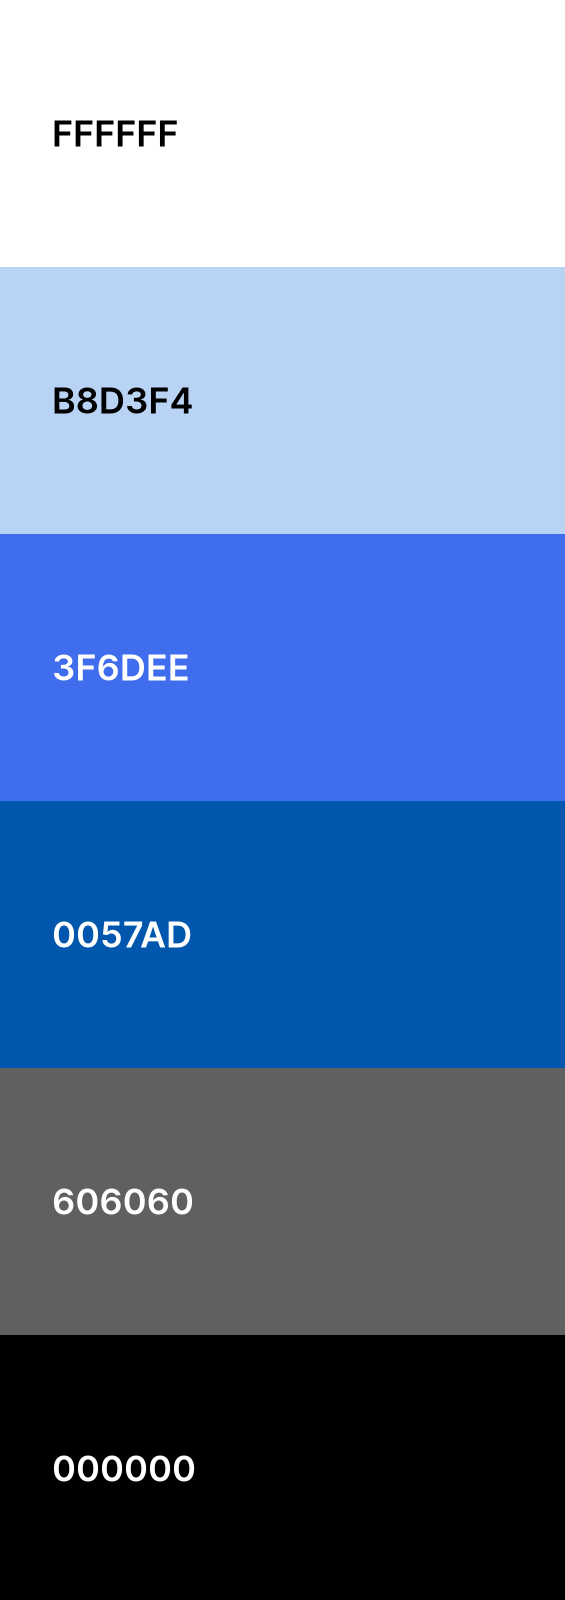
\includegraphics[width=0.2\textwidth]{immagini/palette.png}
    \caption{La principale palette di colori scelta}
\end{wrapfigure}
L'obiettivo di trovare dei colori in contrasto tra loro per gli elementi di testo, background, link, link visitato è stato perseguito utilizzando strumenti come \href{https://webaim.org/resources/contrastchecker/}{WebAIM Contrast Checker}, \href{https://www.audioeye.com/color-contrast-checker/}{ColorAlly (AudioEye)} e \href{https://contrast-finder.tanaguru.com/}{Tanaguru}. Il controllo dei contrasti è stato svolto anche manualmente, sia per evitare falsi positivi, sia per verificare alcuni accostamenti che non vengono recepiti in automatico. Non tutti i colori rappresentati nella palette sono in contrasto tra loro ma gli abbinamenti sono stati scelti con cautela, dato che nel sito c'è una grande preponderanza di bianco. Ad esempio l'azzurro \#B8D3F4, il grigio \#CFCFCF e il bianco non sono in contrasto tra loro, e per questo non sono utilizzati in concomitanza. Sono stati utilizzati diversi colori, nelle immagini e nelle decorazioni, prestando sempre attenzione al loro posizionamento perché vi fosse un contrasto sufficiente. Ci siamo accertati che i colori mantenessero la loro funzionalità anche per gli utenti con daltonismo oppure in visualizzazione in bianco e nero, rispettivamente tramite \href{https://pilestone.com/pages/color-blindness-simulator-1}{Pilestone} e una funzionalità nativa di Windows, Android e iOS.
\subsection{Prestazioni e SEO}
Per assicurare un posizionamento adeguato nei motori di ricerca, oltre che per migliorare l'accessibi\-lità, abbiamo adottato una serie di buone pratiche che coinvolgono sia la struttura del contenuto sia la corretta configurazione del codice HTML.
Un aspetto fondamentale è l'uso appropriato dei tag di intestazione \verb|<h1>, <h2>, ...|: abbiamo garantito che ci sia un solo \verb|<h1>| per pagina, il quale descrive in modo chiaro il contenuto principale, mentre le altre intestazioni (\verb|<h2>, <h3>, ...|) sono utilizzate per suddividere logicamente i paragrafi e migliorare la leggibilità. Anche la scelta delle keywords e la loro inclusione nei meta-tag, come \verb|<meta name="description">|, giocano un ruolo cruciale nel migliorare il ranking: abbiamo selezionato termini pertinenti al contenuto, limitando il numero di caratteri utilizzati ed evitando l'uso eccessivo o forzato, che potrebbe invece penalizzare il posizionamento. In parallelo, abbiamo curato le alternative testuali per le immagini, in modo da fornire informazioni utili sia ai motori di ricerca sia a screen reader e altre tecnologie assistive. Ulteriori accortezze comprendono la verifica regolare di eventuali link rotti o circolari, che possono danneggiare l'esperienza utente e ridurre la credibilità del sito, oltre ad evitare l'abuso di \verb|<h1>|, \verb|<strong>| e altri tag semantici.
\section{Gestione errori}
\subsection{Pagine di errore}
Le pagine di errore hanno lo scopo di rassicurare l'utente quando si dovesse trovare in un percorso sbagliato o dovesse affrontare un problema server-side. In entrambi i casi, le pagine 404 e 500 sono pensate per offrire all'utente un'alternativa simpatica e coerente con lo stile del sito, invitandolo a tornare alla homepage per orientarsi nuovamente.
\subsection{Misure di sicurezza}
La sicurezza dell'applicazione è stata curata in ogni fase di sviluppo, con particolare attenzione ai dati inseriti dagli utenti. Per prevenire potenziali vulnerabilità come l'injection o il cross-site scripting, tutti i dati provenienti dai campi di input vengono sottoposti a un processo di sanitize e validazione lato server, realizzato in PHP. Questo approccio prevede la rimozione o l'escape dei caratteri e delle stringhe potenzialmente pericolose, nonché la verifica della correttezza semantica dei valori inseriti rispetto ai formati o ai tipi di dati previsti. Inoltre è stato implementato un ulteriore controllo lato client, che limita in modo preventivo i caratteri e le parole non consentiti, offrendo all'utente un primo riscontro immediato ed evitando inserimenti scorretti. Tali controlli contribuiscono a migliorare l'esperienza utente e la sicurezza, ma non sostituiscono la validazione server-side, che costituisce la protezione maggiore.
\section{Visualizzazione del sito in ambienti diversi}
Il sito è stato sviluppato in modo da adattarsi a qualunque tipo di device tramite un design fluido implementato con alcuni punti di rottura (breakpoint). Particolare attenzione è stata rivolta alla versione mobile, poiché è plausibile che una buona parte del \hyperref[target]{target} di utenza voglia accedere al sito tramite uno smartphone per ottenere informazioni, contatti o prenotare direttamente una visita.
\subsection{Il sito da desktop, tablet e mobile} \label{desktoptabletmobile}
Nonostante alcune differenze siano già state descritte nel corso della relazione, è importante sottolineare come il sito sia quanto più responsivo possibile, in modo da adattarsi al meglio su ogni dispositivo. Nel passaggio ai layout mobile, la differenza più importante risiede nell'utilizzo del menu ad hamburger al posto delle voci disposte orizzontalmente. Oltre a ciò, cambiano alcuni elementi come la dimensione di testi o immagini e la disposizione in colonna di alcune parti come il footer, le immagini precedentemente affiancate al testo e i box delle news nella homepage. È previsto che l'utente non possa utilizzare alcune interazioni come \verb|hover| e il sito permette un'eguale comprensione di ciò che sta avvenendo, ad esempio tramite il pulsante "torna su". Si vedano infine elementi come i form che subiscono solo modifiche minori per restare centrati e fruibili su ogni dispositivo.
\subsection{Gestione della stampa}
Il layout di stampa è stato ottimizzato per la trasposizione del sito su carta: la versione in bianco e nero mantiene integrità e contrasti, il font diventa con grazie (Times New Roman) e viene giustificato, le immagini decorative non necessarie vengono rimosse. Alcuni layout vengono ripensati, come si può vedere nelle immagini di esempio riportate per la stampa della homepage. L'unico elemento dell'header che rimane è il logo, mentre il footer viene disposto in colonna per ospitare i link completi. In altre pagine, invece, si può trovare una disposizione ulteriormente differente di elementi posti in colonna o dei form che restano intatti dalla loro presentazione su desktop.
\begin{figure} [h]
    \centering
    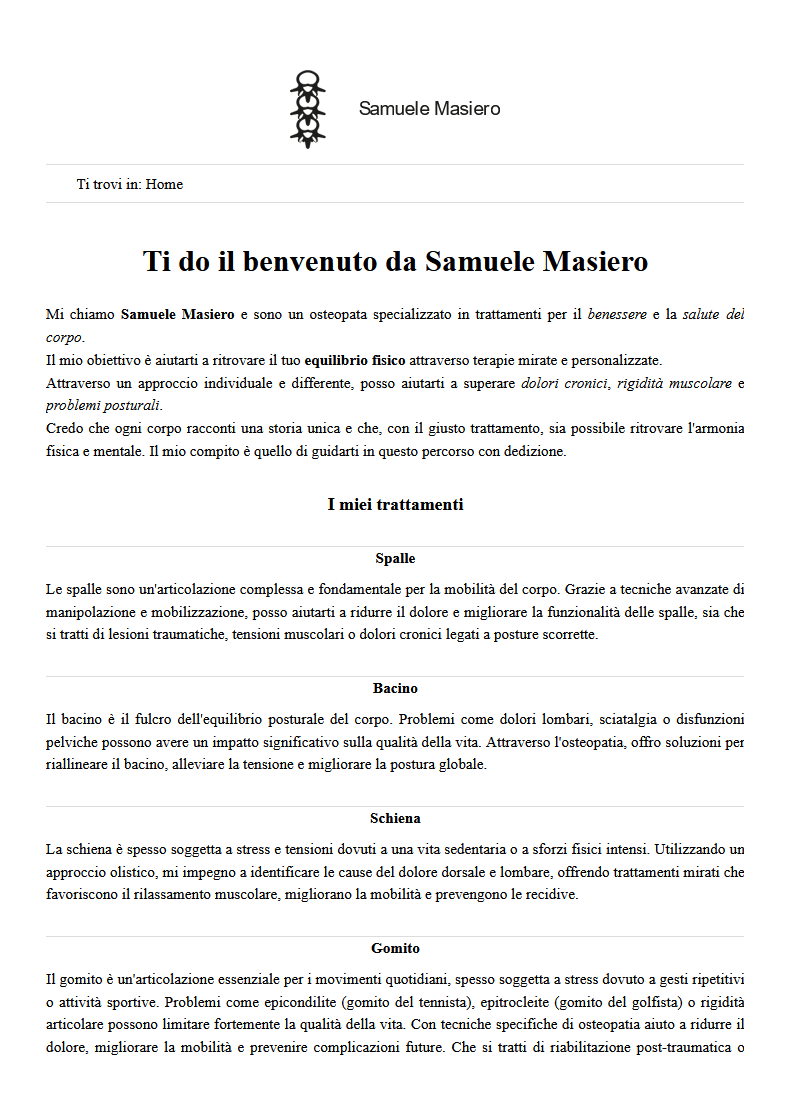
\includegraphics[width=0.4\textwidth]{immagini/print_1.png}
    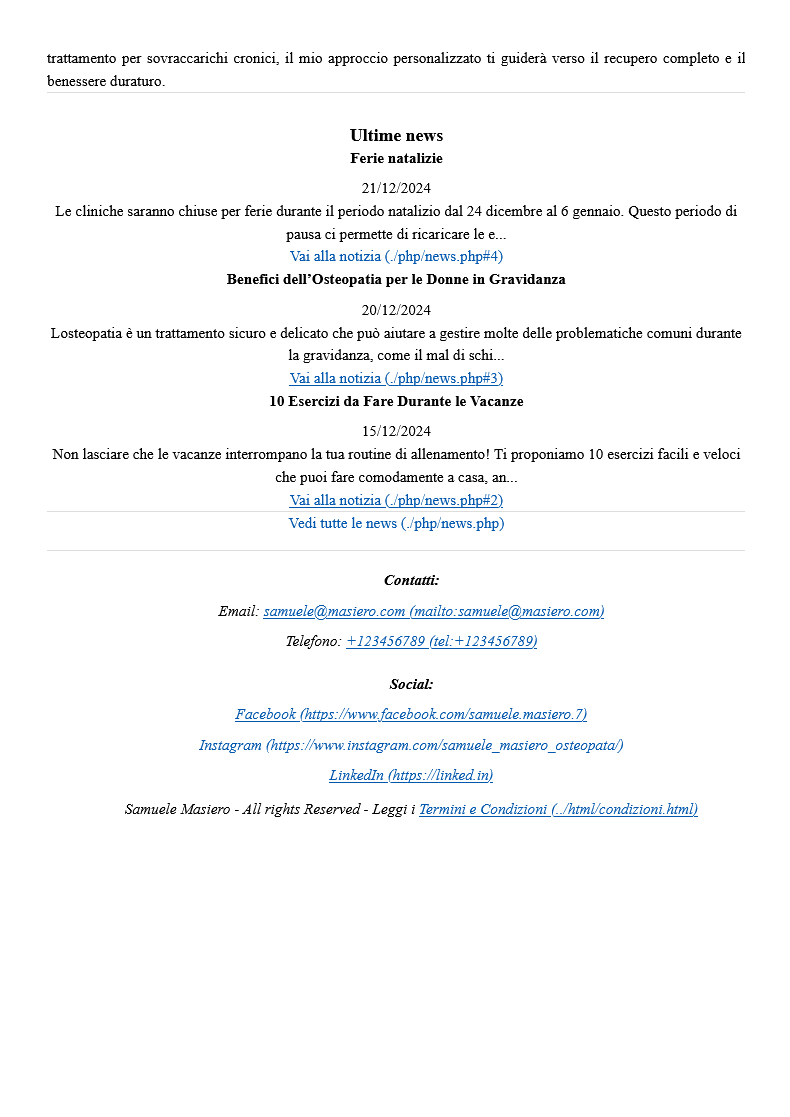
\includegraphics[width=0.4\textwidth]{immagini/print_2.png}
    \caption{Versione di stampa della homepage}
\end{figure}

\end{document}